\externaldocument{main.tex}
As described previously the front-end in this application is a single page application developed with Angular.
This chapter describes the process of integrating Angular with Electron. 
After taking the steps to create and scaffold the Angular application, some configuration work needs to be done.
In the angular.json file the output directory needs to be set to the previously specified directory where 
Electron looks for the index.html file:
\begin{lstlisting}
"options": {
    "outputPath": "dist/pze",
},
\end{lstlisting}
Another modification is required for the start scripts in the package.json file where the angular application has to be built 
and then the electron application:
\begin{lstlisting}
"scripts": {
        "start": "ng build --base-href ./ && electron .",
},
\end{lstlisting}
With this npm start can be executed and first ng build will be called, building the angular application after which the 
Electron start script will be called and the Electron application will be started.\paragraph{}
Now the app is up and running. 
An Electron instance will start with the Angular application running inside it. 
To speed up the development process, the Angular front-end should be developed separately. 
Not only does this lead to looser integration of Angular and Electron but when saving edits made to Angular 
developers need to restart the Electron build process which takes considerably longer than just reloading 
the Angular app. 
This means during development - and as long as the Electron part is not needed - developers should start the 
application with ng serve as changes will be adopted almost instantly whereas with Electron one needs to run the 
entire start script again.\paragraph{}
For communicating between the front- and back-end Electron provides the ipcRenderer and ipcMain modules.
In the front-end part events are emitted with ipcRenderer. 
Electron offers various different ways of sending and receiving events.
The methods to listen to events on the ipcRenderer are as follows: \parencite{electronDocs}
\begin{itemize}
    \item ipcRenderer.on(channel, listener):\\
    This method listens to a channel and when a message on the corresponding 
    channel arrives, the listener is called.
    \item ipcRenderer.once(channel, listener):\\
    Acts similarly to ipcRenderer.on, but the listener is removed after the invocation
\end{itemize}
With ipcRenderer.removeListener(channel, listener) or\\
 ipcRenderer.removeAllListeners(channel) listeners can be removed.
Note that with ipcRenderer.removeAllListeners(channel) the channel parameter is optional and when omitted
all listeners get removed.
The ipcMain Event Emitter has the same methods as ipcRenderer to 
listen to events, with the only addition being ipcMain.handle(channel, listener).\paragraph{}
Similarly to receiving events, Electron offers multiple methods to send events from the ipcRenderer Event Emitter. 
Those methods include: \parencite{electronDocs}
\begin{itemize}
    \item ipcRenderer.send(channel, ...args):\\
     This methods sends an asynchronous message to ipcMain via the specified channel. 
    \item ipcRenderer.invoke(channel, ...args):\\
    This methods also sends an asynchronous message. 
    It does however expect a result and returns a Promise<any> to resolve the response.
    Note that on ipcMain handle() should be used to intercept these events.
    \item ipcRenderer.sendSync(channel, ...args):\\
     Same as ipcRenderer.send(channel, ...args) with the difference of 
    expecting a synchronous result.
    \item ipcRenderer.sendTo(webContentsId, channel, ...args):\\
    A method for sending an event directly to a specified window 
    using the webContentsId parameter.
    \item ipcRenderer.sendToHost(channel, ...args):\\
     Behaves the same as ipcRenderer.send(channel, ...args), with the 
    difference being that the event is sent to the <webview> element rather than the main process.
\end{itemize}
Having listed the options provided by Electron for inter-process communication the next step is to integrate the ipcRenderer into Angular.
For this, there are multiple solutions. 
To simplify development, developers can use an NPM module called ngx-electron developed by Thorsten Hans. \parencite{ngxElectron}
Ngx-electron makes calling Electron's API from Angular simpler for developers by exposing all methods available within Electron's
render process.
This means the above mentioned methods would all be accessible through this module. 
To include it in the Angular application one needs to import the module:
\begin{lstlisting}
import { NgModule } from '@angular/core';
import { BrowserModule } from '@angular/platform-browser';
import { HttpClientModule } from '@angular/common/http';

import { NgxElectronModule } from 'ngx-electron';
@NgModule({
  declarations: [
    AppComponent,
  ],
  imports: [
    BrowserModule,
    BrowserAnimationsModule,
    MaterialModule,
    HttpClientModule,
    NgxElectronModule,
  ],
  bootstrap: [AppComponent],
})
export class AppModule {}
\end{lstlisting}
After then importing the ElectronService class from the ngx-electron module in the necessary components 
one can send or listen to events by accessing the API:
\begin{lstlisting}
this.electronService.ipcRenderer.send('getProjects');
\end{lstlisting}
For this solution to work there is a caveat however: 
If one tries to run this example with the latest stable Electron release (at the time of writing 17.1.0), the 
following error will be encountered:
\begin{lstlisting}
Error: node_modules/ngx-electron/lib/electron.service.d.ts:17:31 - error TS2694: 
Namespace 'Electron.CrossProcessExports' has no exported member 'Remote'.

17     readonly remote: Electron.Remote;
                                 ~~~~~~
\end{lstlisting}
This error occurs because in version 12 of Electron, the remote module has been deprecated and in version 14
removed from Electron itself and moved to another package, @electron/remote. \parencite{electron14Blog}
This of course leads to an error because ngx-electron cannot locate the required module. 
Because the latest release of ngx-electron (version 2.1.1) happened in October of 2019, one can 
assume that this issue (which is still marked as open on GitHub as of March 2022) will not be fixed in 
the foreseeable future. \parencite{namespaceError}
What this means for developers is that if they wish to use ngx-electron, the latest usable stable release
of Electron is 13.6.9. 
While said release was last updated (at the time of writing) on February 2nd 2022, being forced to use
a deprecated feature and being locked into a specific version of any framework can pose a worry to 
many developers. \paragraph{}
As an alternative, developers can skip the use of ngx-electron and directly import the required electron module.
\begin{lstlisting}
const electron = (<any>window).require('electron');
\end{lstlisting}
Sending an event through the ipcRenderer would be very similar to the code sample above which is using 
ngx-electron:
\begin{lstlisting}
// Using ElectronService from ngx-electron
this.electronService.ipcRenderer.send('getProjects');

// Directly accessing ipcRenderer
electron.ipcRenderer.send('getProjects');
\end{lstlisting}
The advantage would be greater future-proofing because the use of a newer Electron stable release would
be possible.
Ultimately which solution is chosen is at the developer's discretion. 
For this proof-of-concept the ngx-electron module will be used.\paragraph{}
In figure six the flow of data is pictured when the application communicates with
the back-end.
One main goal of this application is to take advantage of Electron's arguably biggest asset over 
traditional web applications: offline functionality.
Due to the Electron back-end being developed with Node.js one can access all features available to Node.js 
which in a traditional application would not be accessible on the client's machine.
This means one can use the fact that Electron allows to read and write to the User's file system. 
It is therefore very trivial to implement storage of data on each client's machine.  
See the following sequence diagram for an overview of how data to back up is fetched from the API 
on startup.
\begin{figure}[H]
  \centering
  \label{fig:pze-sequence-diagram-electron}
  \caption{Electron Startup Sequence Diagram:
  A sequence diagram illustrating how data is fetched on startup}
  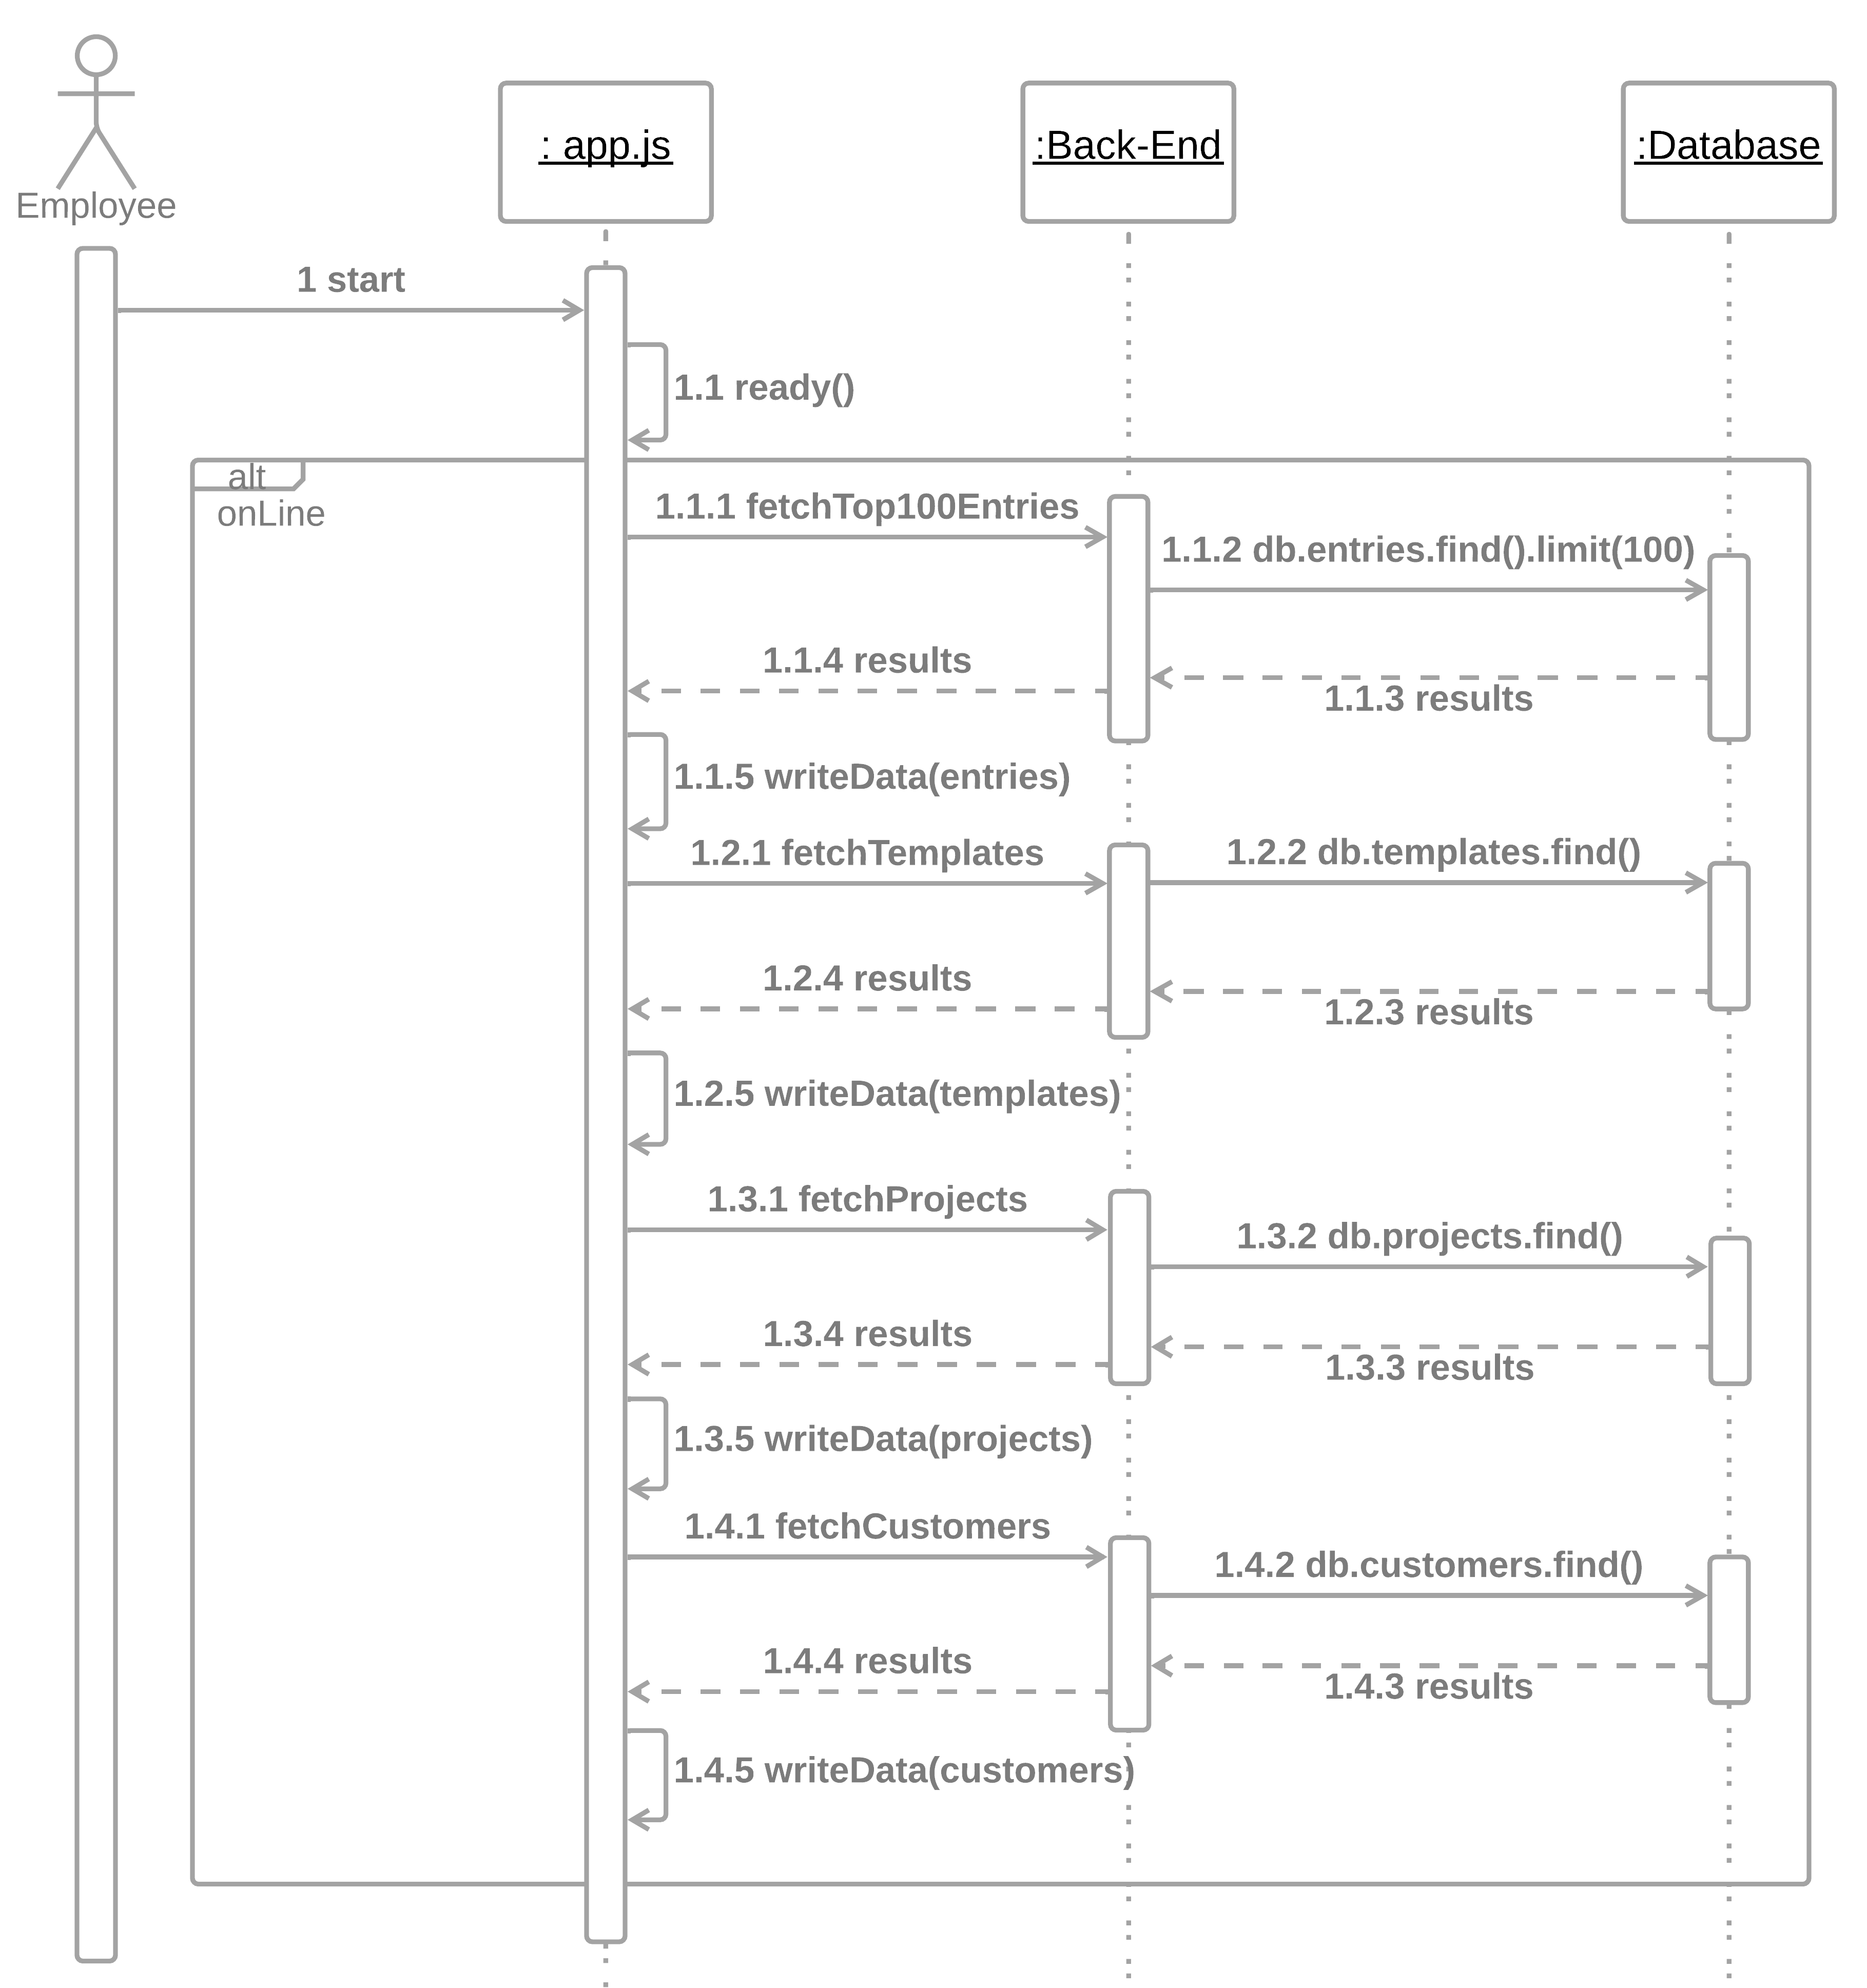
\includegraphics[width=1\textwidth]{pze-sequence-diagram-electron}
\end{figure}
As pictured the API is queried if the application is online.
This is checked via the window.navigator.onLine property 